%! TEX root = ../main.tex

\section{Encuesta de ubicación}
\label{sec:ubicacion}

Para recabar información acerca del nivel de acceso  de los alumnos a la
tecnología, se realiza una encuesta que cuenta con diez preguntas, las cuales
buscan conocer el modelo de dispositivo móvil, el acceso a
Internet, y la predisposición de cada alumno a ayudar en la prueba.

Con los resultados de la encuesta de ubicación tecnológica, se seleccionan
aquellos alumnos que poseen dispositivos móviles que superan o igualan las
especificaciones descritas más adelante. De esta encuesta se obtendrán los 
usuarios que formarán parte de la población que evaluará la versión final de 
la solución.

\subsection{Muestra}

En el año $2014$, el \Gls{iab} cuenta con $124$ alumnos en el cuarto año  de la 
carrera de Licenciatura en Enfermería distribuidos en
tres secciones, estos alumnos son considerados la población objetivo. De los 124, 93 de
ellos estuvieron interesados en completar la encuesta.

\subsection{Variables}

Se definen $3$ factores necesarios para que un alumno pueda ser considerado como
sujeto de prueba, el primero es la predisposición del mismo a participar de la
prueba, el segundo es que posea un dispositivo móvil que supere los requisitos
mínimos explicados más adelante y el tercero es que tenga algún tipo de conexión a 
internet desde el dispositivo móvil pues 
los registros de actividad de cada dispositivo deben ser enviados y almacenados 
para su posterior interpretación y análisis. A continuación se describen las variables 
consideradas.


\begin{itemize}

\item \textbf{Requisitos mínimos:} son aquellos requerimientos técnicos con los que 
    debe cumplir completamente el dispositivo móvil del usuario para que la 
    solución tenga un desempeño que garantice una experiencia fluida a la hora de 
    utilizarla. Estos requisitos son:
    \begin{itemize}
        %%\item Sistema Operativo Android $4.0$ o superior
        \item Memoria ram de $512$MB o superior.
        \item Velocidad de procesador de $800$ GHz o superior.
        \item \Gls{gpu} OpenGL ES 2.0 o superior.
        %\item Conexión frecuente a internet.
    \end{itemize}
    Los requisitos de \textit{hardware} mencionados, son requeridos por las
    características de la simulación, una \Gls{gpu} es requerida por los gráficos en 
    tres dimensiones.

\item \textbf{Tipo de acceso a internet:} el tipo de acceso a internet que posee el 
    usuario en su dispositivo móvil. Puede ser una de las siguientes opciones:
    plan post-pago, paquetes pre-pago, acceso ocasional y sin acceso.
    
\item \textbf{Sistema Operativo:} se refiere al tipo de sistema operativo que posee 
    el dispositivo móvil del usuario.

%    \observacion{Donde se menciona?}
    
\end{itemize}

\subsection{Métricas}

Las métricas utilizadas para estudiar los datos recogidos son sencillas ya que
sólo buscan determinar la población que evaluará la solución, estas métricas son
las siguientes:

\begin{itemize}
\item Porcentaje de encuestados con dispositivos móviles que cumplen y que no cumplen con 
los requisitos mínimos.
\item Porcentaje del tipo de acceso a internet de los encuestados desde sus dispositivos móviles.
\item Porcentaje del tipo de sistema operativo que poseen los dispositivos móviles de los 
encuestados.
\end{itemize}


\subsection{Resultados obtenidos}


%Como se indicó en la sección~\ref{sec:ubicacion}, se agrupa a los
%\fixme{alumnos}{De donde?} encuestados de acuerdo a las características de sus
%dispositivos móviles y del acceso a internet.

%El acceso a internet es un requisito importante, pues para que los mismos puedan
%enviar su progreso y así se registre la utilización de la solución, así, es
%necesario que los usuarios tengan un acceso ocasional a internet. 

En la figura~\ref{fig:ubicacion_acceso_internet} se puede observar que de 93 alumnos 
encuestados, el $94,6\%$ tiene acceso a internet al menos en algún momento y que
solo el $5.4\%$ no tiene acceso a internet en sus dispositivos móviles. Considerando 
sólo estos datos, el $94,6\%$ de los alumnos podría utilizar la solución.

%esto
%permite que tengan acceso a la solución el $94,6\%$ de los alumnos.

%\begin{figure}[H]
%\centering
%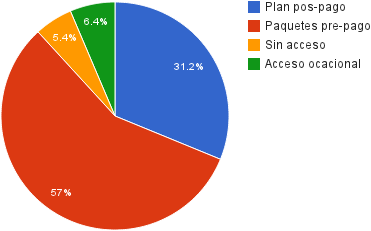
\includegraphics[scale=0.5]{resultados/imagenes/ubicacion_acceso_internet.png}
%\caption{Acceso a internet desde dispositivos móviles}
%\label{fig:ubicacion_acceso_internet}
%\end{figure}

 \begin{figure}[H]
        \centering
        \begin{tikzpicture}[thick,scale=0.7, every node/.style={transform shape}]
            \pie[
                %explode=.2,
                text=legend,
                %style=drop shadow,
                %radius=3,
                %scale font,
                explode={0.1,0.1,0.3,0.3}
                ]%
            {%
                31.2 / Plan pos-pago,
                57   / Paquetes pre-pago,
                5.4  / Sin acceso,
                6.4  / Acceso ocasional}
        \end{tikzpicture}
        \caption{Acceso a internet desde dispositivos móviles}
        \label{fig:ubicacion_acceso_internet}
\end{figure}

%La utilización en dispositivos móviles es un requisito necesario para
%\fixme{la}{Utilizar la solución} solución

Los dispositivos móviles son un requisito para utilizar la solución, 
en la figura\ref{fig:ubicacion_sistemas_operativos} se muestran los sistemas operativos
móviles utilizados por los alumnos encuestados, si bien el motor de videojuego 
utilizado permite generar clientes a diversos sistemas operativos, es importante conocer el sistema
operativo que poseen los alumnos para realizar pruebas.

En la figura~\ref{fig:ubicacion_sistemas_operativos} se puede observar que
\emph{Android} lidera con un $61.3\%$, le sigue Windows Phone con un $12.9\%$.
Si bien, según la tabla~\ref{tab:comparacion_motores_juegos}, \emph{Unity3D}
soporta la mayoría de los sistemas operativos, aún es importante hacer pruebas
sobre un sistema operativo específico. Se selecciona \emph{Android} por ser el
sistema operativo con mayor cuota entre los alumnos.

%\begin{figure}[H]
%\centering
%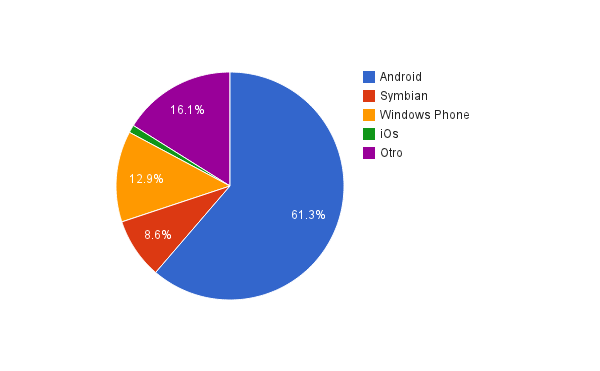
\includegraphics[scale=0.5]{resultados/imagenes/ubicacion_sistemas_operativos.png}
%\caption{Sistemas operativos móviles utilizados}
%\label{fig:ubicacion_sistemas_operativos}
%\end{figure}

 \begin{figure}[H]
        \centering
        \begin{tikzpicture}[thick,scale=0.7, every node/.style={transform shape}]
            \pie[
                text=legend,
                rotate=61.3,
                explode={.1,.2,.2,.2}
                ]%
            {%
            61.3 / Android,
             8.6 / Symbian,
            12.9 / Windows Phone,
            17.2 / Otros}
        \end{tikzpicture}
        \caption{Sistemas operativos móviles utilizados}
	    \label{fig:ubicacion_sistemas_operativos}
\end{figure}
    

Por último, se divide a los encuestados para determinar cuantos de ellos
tiene dispositivos móviles que cumplen los requisitos mínimos para utilizar la
solución propuesta según lo descrito en la sección~\ref{sec:ubicacion}. En la
figura~\ref{fig:ubicacion_requisitos_minimos} se puede observar que el $18,3\%$
de los encuestados cumplen con los requisitos.

Si bien los requisitos de la solución no son elevados para los estándares
actuales, la figura~\ref{fig:ubicacion_requisitos_minimos} nos muestra que el
$18.3\%$ tiene dispositivos de alta gama, el cual es un porcentaje mayor al
esperado. Se observa además que cerca del
$90\%$ posee un dispositivo de gama media o superior, la penetración de los
dispositivos móviles es muy alta en los estudiantes de enfermería del \Gls{iab}.

%\begin{figure}[H]
%\centering
%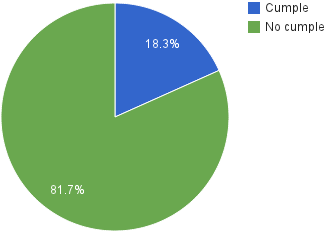
\includegraphics[scale=0.5]{resultados/imagenes/ubicacion_requisitos_minimos.png}
%\caption{Dispositivos que cumplen con los requisitos mínimos para la prueba}
%\label{fig:ubicacion_requisitos_minimos}
%\end{figure}

\begin{figure}[H]
       \centering
       \begin{tikzpicture}[thick,scale=0.7, every node/.style={transform shape}]
           \pie[
                text=legend,
                explode=.1
                ]%
            {%
                81.7 /  No Cumple,
                18.3 /  Cumple
            }
        \end{tikzpicture}
        \caption{Dispositivos que cumplen con los requisitos mínimos para la prueba}
		\label{fig:ubicacion_requisitos_minimos}
\end{figure}

Considerando los datos mostrados, el $17$ alumnos cumplen con los requisitos para utilizar y evaluar 
la solución.



